\clearpage
\chapter{GIỚI THIỆU ĐỀ TÀI VÀ LỰA CHỌN CÔNG NGHỆ}

\section{Giới thiệu đề tài}

\subsection{Lý do chọn đề tài}

Ký túc xá là một bộ phận hỗ trợ trực tiếp đời sống học tập của sinh viên. Trong quá trình vận hành, cán bộ phải theo dõi số lượng phòng và giường, tiếp nhận nhu cầu ở nội trú, bố trí chỗ ở, lập hợp đồng, ghi nhận các khoản phí và xử lý việc trả phòng. Những nghiệp vụ này liên kết chặt chẽ với nhau vì một thay đổi ở trạng thái giường có thể ảnh hưởng đến kết quả tìm phòng, yêu cầu đặt phòng, hợp đồng và khả năng tiếp nhận sinh viên mới.

Khi dữ liệu được ghi chép ở nhiều sổ hoặc tệp riêng lẻ, cán bộ khó xác định trạng thái phòng tại cùng một thời điểm. Một giường có thể đã được giữ nhưng vẫn xuất hiện trong danh sách còn chỗ, hợp đồng đã kết thúc nhưng trạng thái giường chưa được cập nhật, khoản phí đã thanh toán nhưng thông tin chưa được phản ánh kịp thời. Các sai lệch này làm tăng thời gian đối chiếu và có thể dẫn đến bố trí trùng chỗ hoặc cung cấp thông tin không chính xác cho sinh viên.

Sinh viên cũng cần một kênh thống nhất để tìm phòng phù hợp, gửi yêu cầu đặt phòng, theo dõi khoản phí và đề nghị trả phòng. Nếu mỗi nghiệp vụ được xử lý qua một hình thức khác nhau, sinh viên khó biết yêu cầu đang ở bước nào và cần liên hệ với bộ phận nào. Vì vậy, đề tài Hệ thống quản lý ký túc xá PTIT được lựa chọn nhằm xây dựng một quy trình xuyên suốt, trong đó dữ liệu của giai đoạn trước trở thành cơ sở cho giai đoạn sau nhưng mỗi chức năng vẫn có ranh giới xử lý riêng.

Đề tài phù hợp với nội dung học phần Phân tích và thiết kế hệ thống thông tin vì chứa nhiều đối tượng nghiệp vụ có quan hệ rõ ràng như sinh viên, phòng, giường, yêu cầu đặt phòng, hợp đồng, khoản phí và yêu cầu trả phòng. Hệ thống cũng có các quy tắc cần kiểm soát, chẳng hạn không giữ một giường cho nhiều sinh viên trong cùng thời gian, không lập hai hợp đồng còn hiệu lực cho một sinh viên và không giải phóng giường trước khi hoàn tất trả phòng.

\subsection{Mục tiêu của đề tài}

Mục tiêu tổng quát của đề tài là xây dựng mô hình hệ thống thông tin hỗ trợ quản lý vòng đời chỗ ở của sinh viên tại ký túc xá. Hệ thống cần tạo ra một nguồn dữ liệu thống nhất để sinh viên và cán bộ sử dụng theo đúng quyền hạn, giảm thao tác đối chiếu thủ công và duy trì trạng thái phòng, giường, hợp đồng và khoản phí nhất quán.

Các mục tiêu cụ thể gồm:

\begin{itemize}[leftmargin=1.4em]
\item Cung cấp thông tin phòng và giường còn khả dụng để sinh viên tìm kiếm theo nhu cầu thực tế.
\item Ghi nhận yêu cầu đặt phòng và hỗ trợ cán bộ giữ một chỗ cụ thể cho sinh viên.
\item Hỗ trợ lập hợp đồng và xác nhận bàn giao phòng theo các điều kiện đã xác định.
\item Theo dõi khoản phí nội trú và ghi nhận kết quả thanh toán của sinh viên.
\item Tiếp nhận yêu cầu trả phòng, kết thúc hợp đồng và giải phóng giường theo đúng quy trình.
\item Tạo cơ sở dữ liệu đủ nhất quán để phục vụ tra cứu, kiểm tra và mở rộng báo cáo sau này.
\end{itemize}

\subsection{Kết quả dự kiến}

Kết quả của đề tài gồm bộ mô hình phân tích, bộ mô hình thiết kế và một phiên bản hệ thống có thể minh họa các nghiệp vụ chính. Phần phân tích xác định tác nhân, yêu cầu, đặc tả Use Case, biểu đồ hoạt động và lớp nghiệp vụ. Phần thiết kế trình bày kiến trúc, biểu đồ tuần tự, lớp thiết kế, cơ sở dữ liệu và giao diện. Sản phẩm cài đặt cần thể hiện được luồng dữ liệu xuyên suốt từ tạo phòng đến hoàn tất trả phòng.

Về nghiệp vụ, hệ thống dự kiến duy trì được trạng thái của phòng và giường theo từng giai đoạn; lưu được yêu cầu đặt phòng, hợp đồng và khoản phí; đồng thời cung cấp phản hồi rõ ràng khi một yêu cầu không đáp ứng điều kiện. Về mặt học phần, các kết quả này cho phép nhóm kiểm chứng tính nhất quán giữa yêu cầu, mô hình UML, thiết kế dữ liệu và chức năng được cài đặt.

\section{Đối tượng sử dụng và phạm vi hệ thống}

\subsection{Đối tượng sử dụng}

Hệ thống xác định hai tác nhân trong phạm vi hiện tại. Sinh viên là người có nhu cầu tìm và sử dụng chỗ ở. Cán bộ quản lý ký túc xá chịu trách nhiệm cập nhật tài nguyên phòng, xử lý việc bố trí chỗ ở, lập hợp đồng, bàn giao và kết thúc quá trình lưu trú.

\begin{table}[H]
\centering
\small
\caption{Các tác nhân trong phạm vi hệ thống}
\label{tab:ch1-1}
\begin{tabularx}{\textwidth}{|>{\raggedright\arraybackslash}p{0.32\textwidth}|>{\raggedright\arraybackslash}X|}
\hline
\textbf{Tác nhân} & \textbf{Vai trò trong phạm vi} \\
\hline
Sinh viên & Tra cứu phòng còn chỗ, gửi yêu cầu đặt phòng, thanh toán phí nội trú và gửi yêu cầu trả phòng. \\
\hline
Cán bộ quản lý ký túc xá & Tạo phòng và giường giữ chỗ, lập hợp đồng, xác nhận bàn giao và hoàn tất trả phòng \\
\hline
\end{tabularx}
\end{table}

\subsection{Phạm vi chức năng}

Phạm vi được tổ chức theo năm giai đoạn của vòng đời chỗ ở. Mỗi giai đoạn gồm hai chức năng có kết quả riêng. Cách chia này giúp nhóm phân công theo nghiệp vụ mà vẫn giữ được thứ tự chung của hệ thống. Danh sách chức năng trong Bảng 1.1 là phạm vi chính thức dùng cho các chương phân tích, thiết kế và cài đặt.

\begin{table}[H]
\centering
\small
\caption{Phạm vi mười chức năng của hệ thống}
\label{tab:ch1-2}
\begin{tabularx}{\textwidth}{|>{\raggedright\arraybackslash}p{0.18\textwidth}|>{\raggedright\arraybackslash}X|>{\raggedright\arraybackslash}p{0.22\textwidth}|>{\raggedright\arraybackslash}p{0.18\textwidth}|}
\hline
\textbf{Giai đoạn} & \textbf{Mã} & \textbf{Chức năng} & \textbf{Tác nhân} \\
\hline
Xem phòng & UC01 & Cán bộ tạo phòng và giường & Cán bộ \\
\hline
Xem phòng & UC02 & Sinh viên tìm phòng còn chỗ phù hợp & Sinh viên \\
\hline
Đặt phòng & UC03 & Sinh viên gửi yêu cầu đặt phòng & Sinh viên \\
\hline
Đặt phòng & UC04 & Cán bộ giữ phòng và giường cho sinh viên & Cán bộ \\
\hline
Thuê phòng & UC05 & Cán bộ lập hợp đồng thuê phòng cho sinh viên & Cán bộ \\
\hline
Thuê phòng & UC06 & Cán bộ xác nhận bàn giao phòng cho sinh viên & Cán bộ \\
\hline
Đóng phí & UC07 & Cán bộ phát hành khoản phí nội trú theo kỳ & Cán bộ \\
\hline
Đóng phí & UC08 & Sinh viên thanh toán khoản phí nội trú & Sinh viên \\
\hline
Trả phòng & UC09 & Sinh viên gửi yêu cầu trả phòng & Sinh viên \\
\hline
Trả phòng & UC10 & Cán bộ xác nhận hoàn tất trả phòng & Cán bộ \\
\hline
\end{tabularx}
\end{table}

\subsection{Phạm vi dữ liệu}

Hệ thống quản lý các nhóm dữ liệu trực tiếp phục vụ mười chức năng: thông tin sinh viên và cán bộ; tòa nhà, phòng và giường; yêu cầu đặt phòng và dữ liệu giữ chỗ; hợp đồng và bàn giao; khoản phí và giao dịch thanh toán; yêu cầu trả phòng và trạng thái kết thúc lưu trú. Mỗi nhóm dữ liệu phải có trạng thái và thời điểm cập nhật để hệ thống kiểm tra điều kiện trước khi chuyển sang bước tiếp theo.

Dữ liệu danh mục như loại phòng, mức phí, trạng thái giường và kỳ thu được xem là dữ liệu nền. Việc quản trị chi tiết các danh mục này không được tách thành chức năng chính trong phạm vi mười chức năng, nhưng dữ liệu phải tồn tại để các nghiệp vụ tìm phòng, lập hợp đồng và lập khoản phí hoạt động chính xác.

\subsection{Nội dung ngoài phạm vi}

Đề tài chưa xử lý các nghiệp vụ không trực tiếp thuộc vòng đời chỗ ở, gồm quản lý khách ra vào, đăng ký tạm trú với cơ quan nhà nước, quản lý bưu phẩm, sửa chữa cơ sở vật chất, quản lý vật tư, xử lý vi phạm nội trú và thống kê điện nước chi tiết. Các tính năng thông báo nâng cao, tích hợp cổng thanh toán thực tế, ký số hợp đồng và đồng bộ với hệ thống đào tạo cũng được xem là hướng mở rộng.

Việc giới hạn phạm vi giúp nhóm tập trung vào các quan hệ dữ liệu và quy tắc quan trọng nhất. Những chức năng ngoài phạm vi chỉ được đề cập khi cần giải thích một dữ liệu đầu vào hoặc một hướng phát triển; chúng không được đưa vào biểu đồ Use Case tổng quát của phiên bản hiện tại.

\section{Quy trình nghiệp vụ tổng quát}

Quy trình của hệ thống đi theo năm giai đoạn. Các giai đoạn có quan hệ kế tiếp nhưng không đồng nghĩa mọi chức năng phải tự động gọi chức năng tiếp theo. Mỗi chức năng kết thúc bằng một kết quả được lưu, còn người dùng hoặc hệ thống sẽ khởi tạo nghiệp vụ kế tiếp khi đủ điều kiện.

\subsection{Giai đoạn xem phòng}

Cán bộ tạo phòng và các giường thuộc phòng, đồng thời thiết lập những thông tin cần thiết như tòa nhà, loại phòng, sức chứa và trạng thái sử dụng. Sinh viên tìm phòng theo tiêu chí phù hợp. Hệ thống chỉ trả về các phòng có ít nhất một giường khả dụng và đáp ứng điều kiện lọc. Giai đoạn này tạo nguồn dữ liệu phòng chính xác cho việc đặt phòng.

\subsection{Giai đoạn đặt phòng}

Sinh viên chọn phòng phù hợp và gửi yêu cầu đặt phòng. Yêu cầu ghi nhận nhu cầu nhưng chưa làm phát sinh hợp đồng. Sau khi tiếp nhận, cán bộ lựa chọn một phòng và giường cụ thể để giữ cho sinh viên. Trước khi giữ chỗ, hệ thống phải kiểm tra trạng thái giường và xung đột thời gian nhằm tránh một giường được phân cho nhiều người.

\subsection{Giai đoạn thuê phòng}

Khi sinh viên đã có chỗ được giữ hợp lệ, cán bộ lập hợp đồng thuê phòng với thời hạn, mức phí và giường được phân. Việc lập hợp đồng chưa đồng nghĩa sinh viên đã nhận phòng. Cán bộ chỉ xác nhận bàn giao sau khi kiểm tra các điều kiện cần thiết. Khi bàn giao hoàn tất, hợp đồng chuyển sang trạng thái có hiệu lực và giường được xác định là đang thuê.

\subsection{Giai đoạn đóng phí}

Dựa trên hợp đồng và quy tắc thu phí, hệ thống lập khoản phí nội trú cho sinh viên theo từng kỳ. Khoản phí phải thể hiện loại phí, số tiền, hạn thanh toán và trạng thái. Sinh viên lựa chọn khoản phải nộp và thực hiện thanh toán. Hệ thống kiểm tra khoản phí còn hiệu lực, ghi nhận giao dịch và cập nhật trạng thái khi nhận được kết quả hợp lệ.

\subsection{Giai đoạn trả phòng}

Khi không tiếp tục lưu trú, sinh viên gửi yêu cầu trả phòng và cung cấp thời điểm dự kiến. Cán bộ kiểm tra tình trạng hợp đồng và các điều kiện liên quan trước khi xác nhận hoàn tất. Kết quả của bước cuối là hợp đồng kết thúc, sinh viên không còn được ghi nhận đang ở giường đó và giường được chuyển về trạng thái có thể chuẩn bị cho lượt sử dụng tiếp theo.

\subsection{Quan hệ giữa các giai đoạn}

Dữ liệu phòng và giường là nền tảng của toàn bộ quy trình. Kết quả tìm phòng giúp sinh viên lựa chọn nhưng không tự giữ chỗ. Yêu cầu đặt phòng là căn cứ để cán bộ thực hiện giữ chỗ. Dữ liệu giữ chỗ được dùng khi lập hợp đồng; hợp đồng có hiệu lực là cơ sở lập khoản phí và xác định quyền sử dụng giường. Khi trả phòng hoàn tất, trạng thái hợp đồng và giường phải được cập nhật đồng thời để khép kín vòng đời dữ liệu.

Mối quan hệ trên đòi hỏi hệ thống kiểm soát chuyển trạng thái thay vì chỉ lưu các biểu mẫu rời rạc. Một bản ghi không được chuyển sang trạng thái mới nếu điều kiện của giai đoạn trước chưa được đáp ứng. Các quy tắc cụ thể sẽ được trình bày trong Chương II và được hiện thực hóa bằng lớp xử lý, cơ sở dữ liệu và giao diện ở Chương III.

\section{Định hướng giải pháp công nghệ}

\subsection{Giao diện người dùng bằng ReactJS}

ReactJS là thư viện JavaScript dùng để xây dựng giao diện người dùng từ các thành phần độc lập và có thể tái sử dụng. Mỗi thành phần có thể quản lý cách hiển thị, tiếp nhận sự kiện và cập nhật trạng thái tương ứng với một phần của màn hình. Cách tổ chức theo thành phần phù hợp với hệ thống có nhiều biểu mẫu và danh sách lặp lại như phòng, giường, yêu cầu đặt phòng, hợp đồng và khoản phí.

ReactJS được lựa chọn vì hỗ trợ tách giao diện thành các khối nhỏ, giúp nhóm phát triển và kiểm tra từng màn hình thuận lợi hơn. Những thành phần dùng chung như ô tìm kiếm, bảng dữ liệu, biểu mẫu nhập liệu, thông báo trạng thái và hộp xác nhận có thể được sử dụng lại ở nhiều chức năng. Khả năng cập nhật giao diện theo trạng thái cũng phù hợp với các màn hình cần phản ánh kết quả lọc phòng, tình trạng giữ chỗ hoặc trạng thái thanh toán mà không phải tải lại toàn bộ trang.

Trong hệ thống, ReactJS cung cấp hai nhóm giao diện theo quyền sử dụng. Sinh viên có thể tìm phòng còn chỗ, gửi yêu cầu đặt phòng, theo dõi khoản phí, thanh toán và gửi yêu cầu trả phòng. Cán bộ có thể tạo phòng và giường, giữ chỗ, lập hợp đồng, xác nhận bàn giao và hoàn tất trả phòng. ReactJS chỉ thực hiện kiểm tra đầu vào cơ bản và trình bày phản hồi; mọi điều kiện nghiệp vụ có ảnh hưởng đến dữ liệu vẫn được kiểm tra lại tại backend Java.

\begin{figure}[H]
\centering

\includegraphics[width=0.72\textwidth]{assets/image1.png}
\caption{ReactJs}
\label{fig:reactjs}
\end{figure}

\subsection{Backend Java và dịch vụ web}

Java là ngôn ngữ lập trình hướng đối tượng, có hệ thống kiểu dữ liệu chặt chẽ và thư viện hỗ trợ phong phú. Trong kiến trúc dự kiến, Java được sử dụng để xây dựng phần backend chạy trên máy chủ. Thành phần này tiếp nhận yêu cầu từ giao diện ReactJS, xác thực dữ liệu, kiểm tra quyền sử dụng, thực hiện quy tắc nghiệp vụ và phối hợp truy cập PostgreSQL cùng Redis.

Java được lựa chọn vì phù hợp với hệ thống quản lý có nhiều đối tượng nghiệp vụ và mối quan hệ rõ ràng. Các khái niệm như sinh viên, phòng, giường, yêu cầu đặt phòng, hợp đồng, khoản phí và yêu cầu trả phòng có thể được biểu diễn thành các lớp với trách nhiệm riêng. Cơ chế xử lý ngoại lệ và tổ chức mã nguồn theo gói giúp nhóm kiểm soát lỗi, tách các phần của hệ thống và thuận lợi hơn khi nhiều thành viên cùng phát triển rồi hợp nhất sản phẩm.

Backend Java cung cấp các dịch vụ web để giao diện gửi yêu cầu và nhận kết quả dưới dạng dữ liệu có cấu trúc. Backend chịu trách nhiệm kiểm tra lại trạng thái tại thời điểm xử lý, chẳng hạn giường còn khả dụng trước khi giữ chỗ, hợp đồng hợp lệ trước khi bàn giao, khoản phí còn phải thanh toán và hợp đồng đủ điều kiện trước khi trả phòng. Nhờ đó, quy tắc nghiệp vụ không phụ thuộc vào giao diện và vẫn được bảo đảm khi có nhiều yêu cầu truy cập đồng thời.

\begin{figure}[H]
\centering

\includegraphics[width=0.72\textwidth]{assets/image2.png}
\caption{Java}
\label{fig:java}
\end{figure}

\subsection{Cơ sở dữ liệu PostgreSQL}

PostgreSQL là hệ quản trị cơ sở dữ liệu quan hệ được lựa chọn làm nơi lưu trữ dữ liệu chính của hệ thống. Dữ liệu được tổ chức thành các bảng có quan hệ với nhau và được truy vấn bằng SQL. PostgreSQL hỗ trợ khóa chính, khóa ngoại, ràng buộc duy nhất, ràng buộc kiểm tra, chỉ mục và giao dịch, nhờ đó có thể kiểm soát cấu trúc dữ liệu ngay tại tầng cơ sở dữ liệu thay vì chỉ phụ thuộc vào mã nguồn ứng dụng.

PostgreSQL phù hợp với đề tài vì dữ liệu ký túc xá có cấu trúc và liên kết chặt chẽ: một phòng có nhiều giường; sinh viên phát sinh yêu cầu đặt phòng và hợp đồng; hợp đồng làm căn cứ tạo khoản phí; yêu cầu trả phòng gắn với hợp đồng đang hiệu lực. Các ràng buộc quan hệ giúp ngăn bản ghi mồ côi hoặc tham chiếu sai, trong khi ràng buộc duy nhất và chỉ mục hỗ trợ hạn chế dữ liệu trùng và tăng hiệu quả tra cứu theo mã sinh viên, trạng thái phòng hoặc thời hạn hợp đồng.

Những thao tác làm thay đổi nhiều bản ghi được thực hiện trong cùng một giao dịch để bảo đảm nguyên tắc hoàn thành toàn bộ hoặc hủy toàn bộ. Khi xác nhận bàn giao, hệ thống phải đồng thời cập nhật trạng thái hợp đồng và trạng thái giường; khi hoàn tất trả phòng, hợp đồng phải kết thúc và giường phải được giải phóng nhất quán. Nếu một bước thất bại, giao dịch được hủy để PostgreSQL không lưu trạng thái trung gian gây mâu thuẫn dữ liệu.

\begin{figure}[H]
\centering
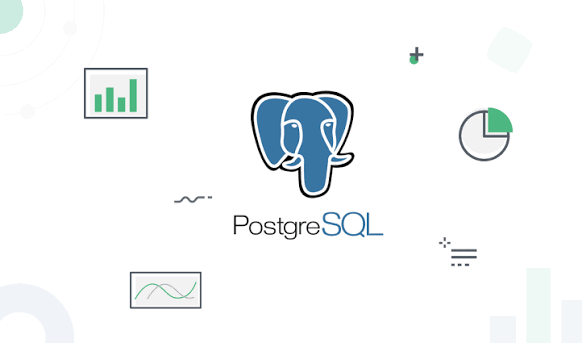
\includegraphics[width=0.72\textwidth]{assets/image3.png}
\caption{PosgreSql}
\label{fig:postgresql}
\end{figure}

\subsection{Sử dụng Redis hỗ trợ tra cứu và giữ giường}

Redis là kho dữ liệu hoạt động chủ yếu trong bộ nhớ và hỗ trợ truy xuất theo khóa với độ trễ thấp. Redis cho phép đặt thời gian tồn tại cho dữ liệu và thực hiện một số thao tác cập nhật có điều kiện, vì vậy phù hợp với thông tin tạm thời hoặc cần phản hồi nhanh. Redis không thay thế PostgreSQL mà đóng vai trò hỗ trợ cho một số tình huống cụ thể của hệ thống.

Redis được lựa chọn nhằm giảm các truy vấn lặp lại và hỗ trợ kiểm soát cạnh tranh khi nhiều người dùng thao tác gần cùng thời điểm. Đối với UC02, hệ thống có thể lưu tạm kết quả tìm phòng còn chỗ trong thời gian ngắn. Khi phòng hoặc giường thay đổi trạng thái, dữ liệu lưu tạm phải được làm mới hoặc loại bỏ để kết quả hiển thị không bị lỗi thời.

Đối với UC04, Redis có thể tạo khóa giữ giường có thời hạn. Backend chỉ tạo khóa khi giường chưa có khóa hợp lệ; khóa tự hết hạn nếu quy trình không được hoàn tất trong thời gian quy định. Cơ chế này giúp hạn chế hai yêu cầu đồng thời cùng giữ một giường, nhưng kết quả cuối cùng vẫn phải được backend kiểm tra và ghi nhận bằng giao dịch trong PostgreSQL. Nếu Redis tạm thời không khả dụng, hệ thống vẫn phải ưu tiên tính đúng đắn của dữ liệu chính và không xác nhận giữ chỗ chỉ dựa trên dữ liệu lưu tạm.

\subsection{Mô hình hóa bằng UML}

UML được sử dụng để mô tả hệ thống ở cả hai pha. Trong pha phân tích, biểu đồ Use Case, biểu đồ hoạt động và biểu đồ lớp phân tích thể hiện yêu cầu và đối tượng nghiệp vụ. Trong pha thiết kế, biểu đồ tuần tự và biểu đồ lớp thiết kế mô tả sự phối hợp giữa giao diện, lớp điều khiển, lớp xử lý nghiệp vụ và lớp truy cập dữ liệu. Việc tách hai pha giúp tránh đưa chi tiết công nghệ vào mô hình nghiệp vụ quá sớm.

\subsection{Công cụ phát triển và quản lý phiên bản}

Nhóm sử dụng công cụ mô hình hóa để xây dựng và thống nhất các biểu đồ UML, công cụ thiết kế giao diện để chuẩn bị bố cục màn hình, môi trường lập trình để cài đặt và hệ thống quản lý phiên bản để lưu vết thay đổi. Tên lớp, mã Use Case và thuật ngữ nghiệp vụ cần được sử dụng nhất quán trong tài liệu, mã nguồn và cơ sở dữ liệu để giảm sai lệch khi các thành viên gộp sản phẩm.
